\documentclass[12pt]{article}
%\usepackage{epsf,epic,eepic,eepicemu}
%\documentstyle[epsf,epic,eepic,eepicemu]{article}
%\usepackage[cp1250]{inputenc}
\usepackage[utf8]{inputenc}
\usepackage{verbatim}
\usepackage{graphicx}

\begin{document}
%\oddsidemargin=-5mm \evensidemargin=-5mm \marginparwidth=.08in
%\marginparsep=.01in \marginparpush=5pt \topmargin=-15mm
%\headheight=12pt \headsep=25pt \footheight=12pt \footskip=30pt
%\textheight=25cm \textwidth=17cm \columnsep=2mm \columnseprule=1pt
%\parindent=15pt\parskip=2pt

\begin{center}
\bf Semestrální projekt MI-PAR 2010/2011:\\[5mm]
    Paralelní algoritmus pro řešení problému: Minimálně lomená souvislá čára\\[5mm]
       Tomáš Čejka\\
	   Martin Lukáš\\[2mm]
magisterské studijum, FIT ČVUT, Kolejní 550/2, 160 00 Praha 6\\[2mm]
\today
\end{center}

\section{Definice problému a popis sekvenčního algoritmu}
Práce se zabývá algoritmem pro konstrukci souvislé lomené čáry skládající se z posloupnosti navazujících úseček, která spojí všech k bodů a bude obsahovat minimum zlomových bodů. 
Sekvenční algoritmus je typu BB-DFS s hloubkou prohledávaného prostoru omezenou na k-2. Řešení vždy existuje.

Vstupní a výstupní jsou téměř stejného formátu. Body jsou v souboru reprezentovány dvěmi celými čísly na řádce. U vstupního souboru je navíc na prvním řádku uveden celkový počet čtených bodů, na pořadí bodů nezáleží. U výstupního souboru na pořadí bodů záleží, jejich pořadí udává posloupnost bodů z nichž je konstruován graf lomené čáry.

Pro reprezentaci bodu načteného ze souboru byla vytvořena třída Point. Objekty této třídy jsou uloženy v globálně přístupném dynamicky vytvořeném poli, jehož velikost je rovněž zachycena v globální proměnné.

Při rekurzivním procházení stavového prostoru byl využit implicitní zásobník pro ukládání zpracovávaných stavů. Tento zásobník je tvořen datovou strukturou std::list ze standartní C++ knihovny. Stavy jsou reprezentovány třídou State, jež uchovává pole celočíselných indexů používaných k adresaci v poli načtených bodů. Tato třída také obsahuje operace např. pro expandování stavu na zásobník. 

Expanze je metoda stavu, která vytváří následníky stavu přidáním doposud nepoužitého bodu. Tímto postupem lze rekurzivně generovat kompletní stavový prostor, všechny permutace pořádí bodů. 

Expanduje se vždy stav z vrcholu zásobníku. Při expanzi stavu se počítá cena, nebo-li počet zlomů vytvořených spojením posloupnosti bodů na než ukazují indexy stavu. Tato cena je taktéž součástí stavu, tedy není nutné opakovaně počítat počet zlomů celé čáry, ale pouze vždy při expanzi rozhodnout o inkrementaci ceny.

Pokud stav nelze již expandovat, je porovnána globální minimální cena s nově vypočtenou hodnotou a případně uchováno řešení s aktualizací globálního minima. Během odebírání stavů ze zásobníku je porovnána cena odebraného stavu s globálním minimem, pak je stav dále expandován nebo je smazán.

Pořadí procházení stavů není nijak měněno, tj. stavy nejsou na zásobníku seřazeny dle ceny, i když by to bylo zřejmně vhodné.

Po vyprázdnění implicitního zásobníku je proveden výpis řešení a program je ukončen.


\section{Popis paralelního algoritmu a jeho implementace v MPI}

\begin{comment} 
rozdělování zásobníku, 
přidělování práce, 
šíření nejlepších výsledků,
ukončovací algoritmus (ADUV)
\end{comment}

\section{Naměřené výsledky a vyhodnocení}
Měření probíhalo za použitím knihovních funkcí OpenMPI. Konkrétně se jednalo o funkce MPI\_Barrier(), 
která nám zaručila synchronizaci všech procesorů, a funkci MPI\_Wtime(), která vrací čas v sekundách.
Čas výpočtu jsme změřili jako rozdíl časů \(t_2\) a \(t_1\), kde \(t_1\) je čas před započetím výpočtu
tesně za inicializací knihovny OpenMPI a \(t_2\) je čas na konci výpočtu před ukončením práce s knihovou.

Část kódu po inicializaci:
\begin{verbatim}
 MPI_Barrier(MPI_COMM_WORLD);
 t1 = MPI_Wtime();
\end{verbatim}
Část kódu před ukončením:
\begin{verbatim}
 MPI_Barrier(MPI_COMM_WORLD);
 t2 = MPI_Wtime();
 if (cpu_id == CPU_MASTER) {
      std::cout << "Spotrebovany cas: " << t2 - t1 << std::endl;
 }
\end{verbatim}

\begin{figure}
\caption{Propojovací síť Ethernet}
\begin{tabular}{|r|r|r|r|}
\hline
Počet CPU & A & B & C\\
\hline
1 & 321,8 & 307,3 & 338,6\\
\hline
2 & 39,46390 & 36,33120 & 40,27212\\
\hline
4 & 13,18690 & 12,84250 & 21,87080\\
\hline
8 & 7,81430 & 10,90410 & 15,13350\\
\hline
16 & 7,51740 & 8,99971 & 11,43290\\
\hline
24 & 37,14640 & 7,44230 & 9,58400\\
\hline
32 & 6,92410 & 7,53790 & 9,39125\\
\hline
\end{tabular} 
\end{figure}

\begin{figure}
 \caption{Propojovací síť InfiBand}
\begin{tabular}{|r|r|r|r|}
\hline
Počet CPU & A & B & C\\
\hline
1 & 321,8 & 307,3 & 338,6\\
\hline
2 & 38,95370 & 35,46150 & 40,27100\\
\hline
4 & 12,20080 & 12,45520 & 21,30230\\
\hline
8 & 7,14178 & 10,43290 & 15,05280\\
\hline
16 & 6,55517 & 8,99971 & 11,43290\\
\hline
24 & 6,21340 & 7,14230 & 8,85400\\
\hline
32 & 6,24150 & 7,13790 & 8,42100\\
\hline
\end{tabular} 
\end{figure}

\begin{figure}
 \caption{Zrychlení Propojovací síť InfiBand}
\begin{tabular}{|r|r|r|r|}
\hline
Počet CPU & A & B & C\\
\hline
1 & 1 & 1 & 1\\
\hline
2 & 8,26 & 9,00 & 8,99\\
\hline
4 & 26,38 & 25,61 & 16,99\\
\hline
8 & 45,06 & 30,58 & 24,05\\
\hline
16 & 49,09 & 35,45 & 31,66\\
\hline
24 & 51,79 & 44,66 & 40,89\\
\hline
32 & 51,56 & 44,69 & 42,99\\
\hline
\end{tabular} 
\end{figure}

\begin{figure}
 \caption{Zrychlení Propojovací síť Ethernet}
\begin{tabular}{|r|r|r|r|}
\hline
Počet CPU & A & B & C\\
\hline
1 & 1 & 1 & 1\\
\hline
2 & 8,15 & 8,78 & 8,99\\
\hline
4 & 24,40 & 24,84 & 16,55\\
\hline
8 & 41,18 & 29,26 & 23,92\\
\hline
16 & 42,81 & 35,45 & 31,66\\
\hline
24 & 45,03 & 42,86 & 37,77\\
\hline
32 & 46,48 & 42,32 & 38,55\\
\hline
\end{tabular} 
\end{figure}

\section{Závěr}
Zhodnocení

\section{Literatura}

\appendix
\begin{figure}[ht]
\begin{center}
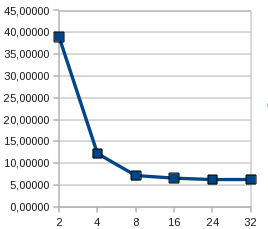
\includegraphics[width=8cm]{grafy-zprava/testAinfib.png}
\caption{Graf závislosti času na počtu CPU test A, InfiBand}
\label{fig:testAinfib}
\end{center}
\end{figure}

\end{document}
